\documentclass[12pt,a4paper]{article}
%\usepackage{fontspec, xunicode, xltxtra}  
%\setmainfont{Hiragino Sans GB}  
%\usepackage{xeCJK}
%\setCJKmainfont[BoldFont=STZhongsong, ItalicFont=STKaiti]{STSong}
%\setCJKsansfont[BoldFont=STHeiti]{STXihei}
%\setCJKmonofont{STFangsong}

%使用Xelatex编译

% 设置页面
%==================================================
\linespread{2} %行距
% \usepackage[top=1in,bottom=1in,left=1.25in,right=1.25in]{geometry}
% \headsep=2cm
% \textwidth=16cm \textheight=24.2cm
%==================================================

% 其它需要使用的宏包
%==================================================
\usepackage[colorlinks,linkcolor=blue,anchorcolor=red,citecolor=green,urlcolor=blue]{hyperref} 
\usepackage{tabularx}
\usepackage{authblk}         % 作者信息
\usepackage{algorithm}     % 算法排版
\usepackage{amsmath}     % 数学符号与公式
\usepackage{amsfonts}     % 数学符号与字体
\usepackage{mathrsfs}      % 花体
\usepackage{amssymb}
\usepackage[framemethod=TikZ]{mdframed}
\usepackage{extarrows}

\usepackage{graphicx} 
\usepackage{graphics}
\usepackage{color}
\usepackage{xcolor}
\usepackage{tcolorbox}
\usepackage{lipsum}
\usepackage{empheq}

\usepackage{fancyhdr}       % 设置页眉页脚
\usepackage{fancyvrb}       % 抄录环境
\usepackage{float}              % 管理浮动体
\usepackage{geometry}     % 定制页面格式
\usepackage{hyperref}       % 为PDF文档创建超链接
\usepackage{lineno}          % 生成行号
\usepackage{listings}        % 插入程序源代码
\usepackage{multicol}       % 多栏排版
%\usepackage{natbib}         % 管理文献引用
\usepackage{rotating}       % 旋转文字,图形,表格
\usepackage{subfigure}    % 排版子图形
\usepackage{titlesec}       % 改变章节标题格式
\usepackage{moresize}   % 更多字体大小
\usepackage{anysize}
\usepackage{indentfirst}  % 首段缩进
\usepackage{booktabs}   % 使用\multicolumn
\usepackage{multirow}    % 使用\multirow

\usepackage{wrapfig}
\usepackage{titlesec}     % 改变标题样式
\usepackage{enumitem}
\usepackage{aas_macros}
\usepackage{bigints}

\renewcommand{\vec}[1]{\boldsymbol{#1}}
\newcommand{\me}{\mathrm{e}}
\newcommand{\mi}{\mathrm{i}}
\newcommand{\dif}{\mathrm{d}}
\newcommand{\tabincell}[2]{\begin{tabular}{@{}#1@{}}#2\end{tabular}}

\def\kpc{{\rm kpc}}
\def\km{{\rm km}}
\def\cm{{\rm cm}}
\def\TeV{{\rm TeV}}
\def\GeV{{\rm GeV}}
\def\MeV{{\rm MeV}}
\def\GV{{\rm GV}}
\def\MV{{\rm MV}}
\def\yr{{\rm yr}}
\def\s{{\rm s}}
\def\ns{{\rm ns}}
\def\GHz{{\rm GHz}}
\def\muGs{{\rm \mu Gs}}
\def\arcsec{{\rm arcsec}}
\def\K{{\rm K}}
\def\microK{\mu{\rm K}}
\def\sr{{\rm sr}}
\newcolumntype{p}{D{,}{\pm}{-1}}

\renewcommand{\figurename}{Fig.}
\renewcommand{\tablename}{Tab.}

\renewcommand{\arraystretch}{1.5}

\setlength{\parindent}{0pt}  %取消每段开头的空格

\newcounter{theo}[section]\setcounter{theo}{0}
\renewcommand{\thetheo}{\arabic{section}.\arabic{theo}}
\newenvironment{theo}[2][]{%
\refstepcounter{theo}%
\ifstrempty{#1}%
{\mdfsetup{%
frametitle={%
\tikz[baseline=(current bounding box.east),outer sep=0pt]
\node[anchor=east,rectangle,fill=blue!20]
{\strut Theorem~\thetheo};}}
}%
{\mdfsetup{%
frametitle={%
\tikz[baseline=(current bounding box.east),outer sep=0pt]
\node[anchor=east,rectangle,fill=blue!20]
{\strut Theorem~\thetheo:~#1};}}%
}%
\mdfsetup{innertopmargin=10pt,linecolor=blue!20,%
linewidth=2pt,topline=true,%
frametitleaboveskip=\dimexpr-\ht\strutbox\relax
}
\begin{mdframed}[]\relax%
\label{#2}}{\end{mdframed}}

\newcommand*\widefbox[1]{\fbox{\hspace{2em}#1\hspace{2em}}}


\title{Gamma Ray Burst}
\author{}
\date{\today}
\begin{document}

\maketitle

\cite{2015PhR...561....1K} GRBs are irregular pulses of gamma-ray radiation (typically lasting for less than one minute), with a non-thermal (broken power-law) spectrum peaking at $\sim10 - 10^4$ keV, and are seen a few times a day at random locations in the sky. The histogram of GRB duration has two distinct peaks. One at $0.3$ s and the other at about $30$ s, which are separated by a dip at $2$ s. Bursts with duration less than $2$ s are classified as \textcolor{red}{short-GRBs} and those that last for more than $2$ s are called \textcolor{red}{long- GRBs}. Long-GRBs are one possible outcome of the collapses of massive stars (mass $\geqslant 15 M_\odot$), and that at least some of the short-GRBs arise in the mergers of compact objects in binary systems (perhaps merger of two neutron stars or a neutron star and a black hole). GRBs are located at distances much larger than the size of the local group of galaxies. From burst redshift and flux we know that GRBs radiate between $10^{48}$ and $10^{55}$ ergs, if isotropic.

\cite{harwit2006astrophysical} Gamma-ray bursts are short outbursts of gamma rays, in the energy range from $50$ keV to $1$ MeV, generally lasting from a fraction of a second to one hundred seconds. In other energy ranges the bursts have sometimes been observed to last longer. The energy of a burst appears to be beamed into a relatively narrow solid angle. Bursts lasting longer than $2$ s are now known to arrive from remote galaxies and appear to originate in extremely powerful supernova explosions. Short bursts sometimes lasting only a tenth of a second are also observed in distant galaxies, and believed to be emitted in the final merger of two compact stars, a neutron star binary or a neutron-star/black-hole binary, as the stars coalesce as a single black hole. A small handful of GRBs are repeating bursters identified with neutron stars associated with supernova remnants.


When a collapsar explodes with an energy of order $10^{51}$ erg a high-temperature, optically thick electron-positron plasma, called a fireball is created. It expands ultrarelativistically into the ambient medium creating a forward shock in the medium, while, by symmetry, a reverse shock plows into the fireball. The ultrarelativistically expanding front of the fireball is often referred to as a blast wave. 

A variety of processes spring into action at the shock front, including Fermi- acceleration of particles, synchrotron radiation by electrons, and inverse Compton production of high energy $\gamma$-rays created as ambient radiation is scattered off high- energy cosmic-ray electrons. If the shock front moves relativistically in the direction of the observer, the $\gamma$-rays produced at the expanding front are observed to arrive during a highly contracted period. In the rest-frame of the expanding front, the photons may be created over the course of a few days, but at the observer, they arrive within a span of seconds.

Most of GRBs are observed to come from highly red-shifted galaxies. Were it not for their immensely energetic outbursts, and the narrow beams into which the $\gamma$-rays are confined ---  the cone angle of the emitted beam may span no more than a few degrees --- they would probably be missed. As the expansion of the fireball slows down, a lower-energy X-ray and optical afterglow persists, apparently beamed into a considerably wider angle. 



GRBs with durations \textcolor{red}{exceeding $2$ s} appear to originate in \textcolor{red}{hypernova explosions} in distant galaxies. Hypernovae are extremely energetic supernovae. In contrast to more common supernovae that eject material at a few thousand kilometers per second, hypernovae explosively eject matter at initial velocities in excess of $30,000$ km s$^{-1}$. A current model for long-duration GRBs and hypernova explosions postulates that they result from the \textcolor{red}{core collapse of an isolated massive star} --- a \textcolor{red}{core collapse supernova} or \textcolor{red}{collapsar}. As the star collapses a black hole embedded in an accretion disk is formed in its center. Neutrinos emitted from the accretion disk exert an outward pressure on the collapsing star, through absorption, scattering, and the formation of electron/positron pairs and photons in neutrino–antineutrino annihilation. Neutrino annihilation occurs mainly in the innermost regions of the disk, above and below the black hole, and along the rotation axis of the disk.

The neutrino scattering and absorption opacities, $\kappa_{sc}$ and $\kappa_{abs}$, respectively, are
\begin{align}
\kappa_{sc} \sim \dfrac{5\alpha^2 +1}{24} \dfrac{\langle \epsilon_\nu^2\rangle \sigma_0}{(m_e c^2)^2 } \dfrac{\rho}{m_u} (Y_n+Y_p) ~, \\
\kappa_{abs} \sim \dfrac{3\alpha^2 +1}{4} \dfrac{\langle \epsilon_\nu^2\rangle \sigma_0}{(m_e c^2)^2 } \dfrac{\rho}{m_u} (Y_n+Y_p) ~.
\end{align}
$\alpha = -1.26$ is a coupling constant, $\epsilon_\nu$ is the neutrino energy, $\sigma_0 = 1.76 \times 10^{-44}$ cm$^2$, $\rho_0$ is the density of stellar material along the rotation axis above the disk, $m_u = 1.67 \times 10^{-24}$ g is the atomic mass unit, and $Y_n \equiv (n_n/n_b) \sim 0.5$ and $Y_p \equiv n_p/n_b \sim 0.5$ are the number fractions of neutrons and protons, with respect to the total number density of baryons $n_b$.

The neutrinos in the disk are largely produced through capture of degenerate electrons and inverse beta decay, as high electron-degeneracy-pressures, produced in the collapse drive electrons into nuclei. However, antineutrinos can also be produced. The mutual annihilation produces electron-positron pairs and photons which are readily absorbed by the surrounding medium. Onset of the explosion along the rotation axis occurs when the inward-directed gravitational acceleration of the black hole on matter in the collapsing star $a_g = -M_{BH} G/r^2$ is exceeded by the outward-directed acceleration due to neutrino scattering, absorption, and annihilation, $a_g + a_{\nu,sc} + a_{\nu,abs} + a_{\nu, \bar{\nu}} > 0$.

For a star with an initial mass in the range $\sim 40$ to $60 M_\odot$, the rate at which the central black hole accretes mass has been estimated to be between $\sim 0.5-1 M_\odot$ s$^{-1}$, and the mass of the final black hole is thought to be around $14$ to $23 M_\odot$. The accretion energy released as mass from the disk spirals into the black hole, is converted into the explosive energy of a bi-lobed, highly-relativistic jet beamed along the star's poles. The high Lorentz factor $\Gamma(v) \equiv [(1 - (v/c)^2]^{-1/2} \sim 100$ of the ejected jet accounts for a confined angle within which the $\gamma$-emission appears particularly strong. More important, the high value of $\Gamma(v)$ accounts for two other factors --- the high energy of the individual highly Doppler-shifted $\gamma$-photons received, and the short duration of the GRB. The Doppler shift tells us that the energy of the photons arriving at Earth will be Doppler shifted by a factor $\Gamma(v)$. If the duration of emission in the rest-frame of the jet is $\Delta t_{\rm rest}$, the duration of the $\Gamma$-emission for an observer at whom the jet is directed will be $\Delta t_{\rm obs} \sim (1 - v/c) \Delta t_{\rm rest} \sim (1/2)\Gamma(v)^{-2} \Delta t_{\rm rest}$. With a Lorentz factor as high as $\Gamma(v) \sim 100$, $\gamma$-rays emitted by the jet in the course of two days would arrive at Earth within an interval of $10$ s. However, for distant GRBs the cosmic red shift z increases this duration by a factor of $z + 1$. 

GRBs lasting \textcolor{red}{less than $\sim 0.1$ s} in the higher energy $100-400$ keV range have been identified as due to the \textcolor{red}{merger of neutron-star-, black-hole-, or mixed neutron-star/black-hole-binaries to form a single black hole}. 

\cite{weekes2003very} 


\cite{courvoisier2012high} Gamma Ray Bursts (GRBs) are short bursts of gamma rays lasting from \textcolor{blue}{a small fraction of a second} to \textcolor{blue}{a few hundred seconds} that are observed from \textcolor{blue}{random directions of the sky} at a frequency of roughly \textcolor{blue}{once per day}. Bursts are identified as ``GRB yymmdd", where yy stands for the year, mm the month, and dd the day of the event. When more than one burst occurs at any given date a letter is added to distinguish between them. Bursts show a wide variety of light curve shapes and structure. 

The distribution of burst duration shows two maxima, one at about \textcolor{red}{$1$ s} and the other at \textcolor{red}{$100$ s} referred to as \textcolor{red}{short bursts}, and \textcolor{red}{long bursts} respectively. Peak photon fluxes (the maximum measured flux during a burst, a quantity depending on the time resolution of the instruments) are typically measured in a few photons per square centimeter per second. The corresponding energy fluxes are of the order of a few $10^{-8}$ erg s$^{-1}$ cm$^{-2}$ and the fluences (flux integrated over time) of a few $10^{-7}$ erg cm$^{-2}$. 

\cite{weekes2003very} A relativistic fireball originates from a catastrophic event involving the formation of black hole. Three scenarios have been proposed: \\
(1) the \textcolor{red}{merging of two neutron stars} to form a black hole; \\
(2) the core collapse of a massive star ($10 M_\odot$, a so-called \textcolor{red}{hypernova}); \\
(3) a supernova, the collapse of a neutron star into a black hole formed in a supernova explosion. \\
The energy could be extracted from the black hole as it is postulated to happen in an AGN, i.e. the rotational energy is tapped via the \textcolor{yellow}{unipolar inductor mechanism}.

\section{Properties of gamma-ray bursts}
\cite{weekes2003very} Bursts are detected with durations from milliseconds to thousands of seconds in duration. The pulse shapes are highly irregular, some with very smooth light curves, others with detailed time structure. There is evidence for at least two classes of bursts with a break between the two populations at $t = 2$ s. There is sub-structure within the bursts but no consistent pattern; there is no evidence for periodic structure. Rise-times of the overall burst and of substructures within the burst tend to be sharper than fall times. At high energies ($> 30$ MeV), there is evidence for a delayed emission but this may be from a different component in the emission process. 

There is not nearly as wide a variation in behavior with photon energy as there is with time. Almost all the power is emitted at energies \textcolor{blue}{above $50$ keV}. The spectra show no spectral lines and is generally a \textcolor{blue}{smooth continuum}: the distribution of peak energies is surprisingly narrow. The spectra can be represented by two power laws, with differential index from $0$ to $-1.5$ up to the power maximum, and $-2$ to $-2.5$ thereafter. There is some evidence for a change of spectrum during the burst with most bursts softening over their duration.


If the distribution of GRB sources is \textcolor{blue}{homogeneous in space}, i.e. if the \textcolor{blue}{density and luminosity are independent of position within the observable volume}, then the integral intensity distribution will be \textcolor{yellow}{$N(> F) \propto F^{-3/2}$}. There is a clear deviation at lower intensities, possibly indicating that the edge of the distribution in space has been reached.

\begin{figure}
\begin{center}
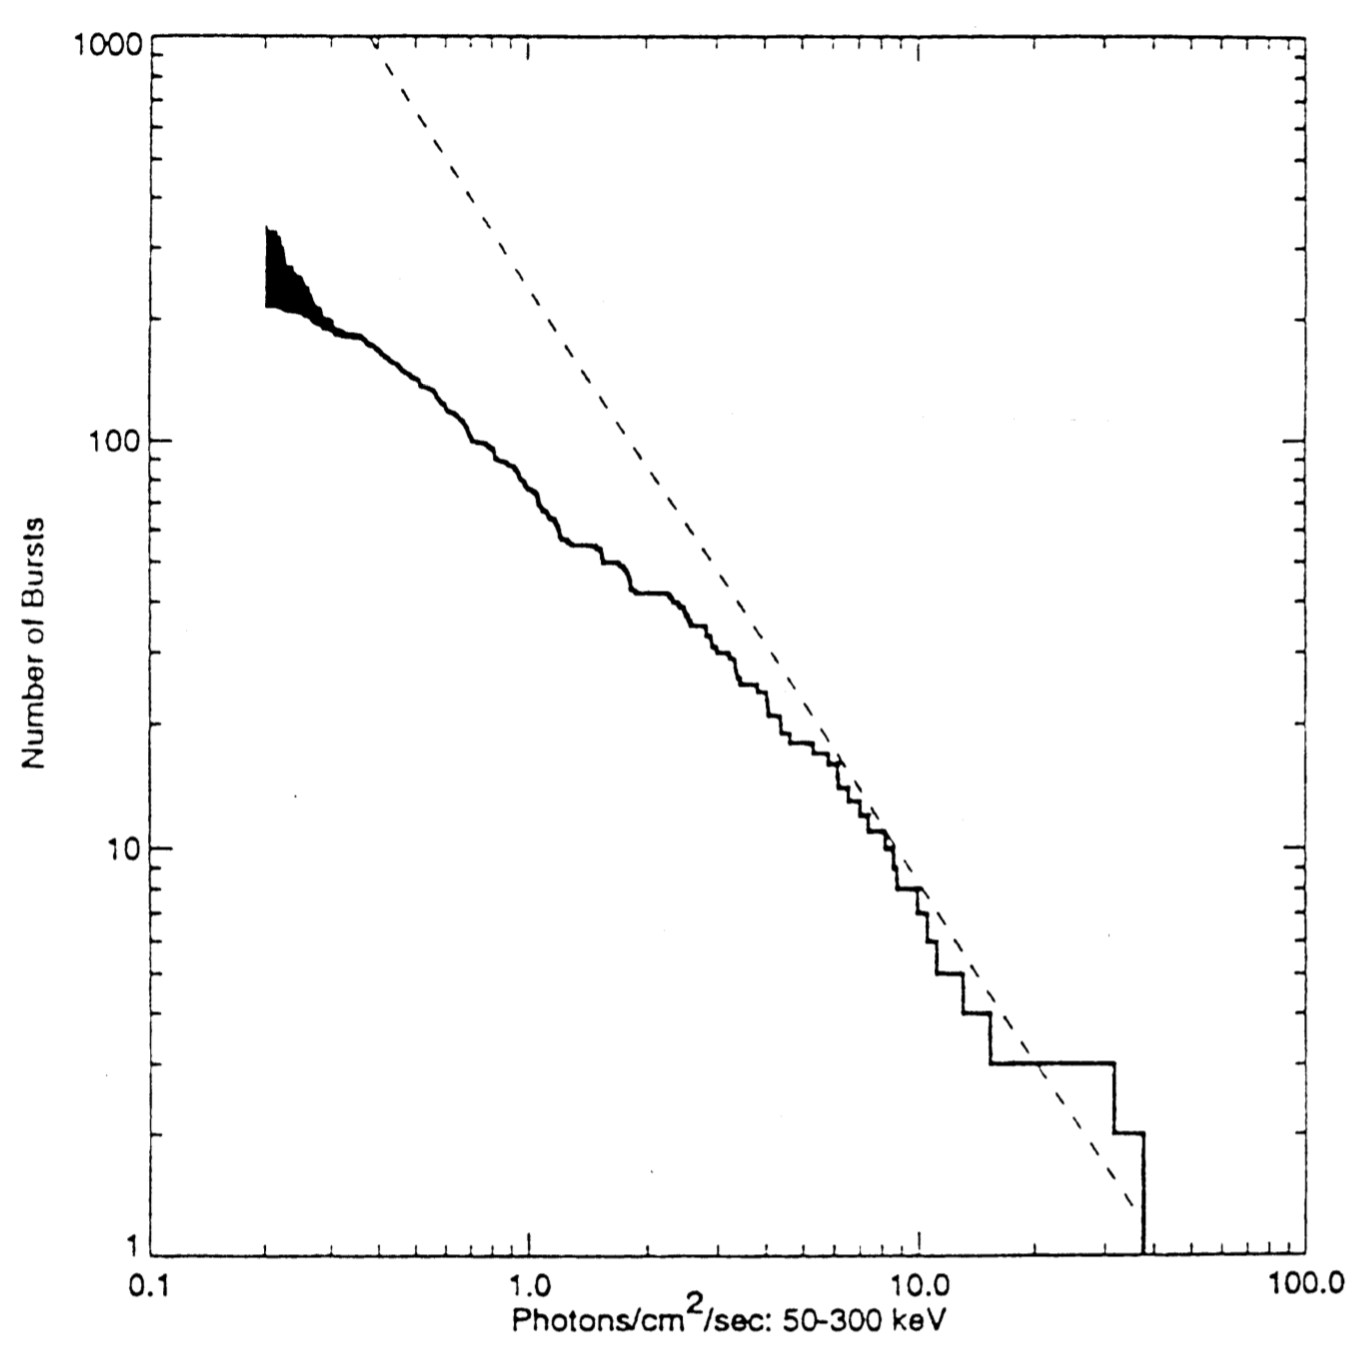
\includegraphics[width=12cm]{GRBdistribution.png}
\caption{Intensity distribution of GRBs showing deviation from the $-3/2$ power law expected if GRBs are homogeneously distributed in Euclidean space. 
}
\label{FIG:synchro_spectrum2}
\end{center}
\end{figure}

\cite{courvoisier2012high}  The expected integral flux distribution of a homogeneous source distribution in Euclidean space is a power law of slope $-3/2$. Consider a density n of sources of luminosity $L_0$. There are $\Delta N = 4\pi r^2 \Delta r n$ sources in a shell of width $\Delta r$ at a distance  $r$ from any observer. The sources in the shell are observed to have a flux $s = \dfrac{L_0}{4\pi r^2}$. They are observed in a flux interval
\begin{equation}
\Delta s = \dfrac{\dif L}{\dif r} \Delta r = \dfrac{-2L_0}{4\pi r^3} \Delta r ~.
\end{equation}
Using $r = \sqrt{\dfrac{L_0}{4\pi s}}$, 
\begin{equation}
\Delta N = 4\pi r^2 \Delta r n = 4\pi \dfrac{L_0}{4\pi s} n \dfrac{4\pi (\sqrt{\dfrac{L_0}{4\pi s}})^3}{2L_0} \Delta s ~.
\end{equation}
The number of sources brighter than a given flux $s$ is 
\begin{equation}
N(s) = \int \dfrac{\Delta N}{\Delta s} \dif s \propto \int s^{-5/2} \dif s \propto s^{-3/2} ~,
\end{equation}
This argument is trivially extended to any distribution of intrinsic source luminosities, as long as the source luminosity distribution does not depend on the distance to the observer.

Some of the physical conditions of the burst emitting matter can be deduced from their implied luminosities and variability timescale. Consider first the optical depth of the emission region. The optical depth for photon-photon $e^+ - e^-$ pair creation close to the threshold is
\begin{equation}
\tau \simeq \dfrac{L}{4\pi m_e c^4 \Delta t} \sigma_T ~,
\end{equation}
where we have assumed spherical symmetry, and where we approximate the size of the source by $c \Delta t$, $\Delta t$ being the variability timescale. For a typical isotropic burst luminosity of $10^{50}$ erg s$^{-1}$ and for a variability timescale of $0.001$ s the optical depth for $e^+ - e^-$ pair creation is $\tau \simeq 6 \times 10^{12}$. This is in clear contradiction with the mere fact that gamma rays are observed. Relativistic aberration effects can, however, bring relief. Imagine that the source is moving towards the observer with relativistic velocities characterized by a factor $\gamma$. The observed flux will be increased by a factor $\gamma^2$ when compared with the flux that would be measured from a source at rest. The variability timescale would also differ by a factor $\gamma$. The pair production rate is reduced by a further factor $\gamma$, because the threshold for pair production is to be considered in the moving reference frame. The optical depth that we would deduce from a source moving towards us would therefore be $\gamma^4$ less than that deduced for a source at rest. We therefore conclude that for a source with the observed properties of gamma ray bursts to be optically thin in the gamma ray domain, a condition necessary for this source to radiate efficiently, the bulk $\gamma$ factor must be at least of order several hundred.

Furthermore, the bursts need not be isotropically emitted but may rather be emitted in a jet geometry. The jet must necessarily be directed towards the observer, and it must cover only a small fraction of the sphere as seen from the object at the origin of the jet. This would reduce the intrinsic luminosity of the source by a factor corresponding to the ratio of the jet solid angle to $4 \pi$.

The very high gamma factor deduced from the optical depth argument implies that the material that emits the burst must be very thinly populated by hadrons. Indeed the photon and lepton flux associated with the moving material (for which the optical depth argument is valid) will accelerate hadrons in the flow to about the same bulk Lorentz factor. If, as can be expected, the kinetic energy luminosity of the jet is similar to the observed photon luminosity, than only a mass of some $m \simeq L \Delta t \simeq 10^{-6} M_\odot$ can be accelerated.

The model that results from these considerations is that some very energetic event, such as the core collapse of a massive star or the merger of two neutron stars or black holes, liberates in a very short time an energy $\simeq 10^{50}$ erg.  This energy generates a very powerful jet in which the bulk γ factor reaches $\simeq 1,000$. Powerful shocks are created in this jet, for example when a faster element follows a slower one. Electrons and positrons are then accelerated in these shocks to very high energies and radiate through synchrotron and Compton processes. This is the radiation that is at the origin of the prompt emission of the burst. The jet then reaches the interstellar matter that surrounds the original explosion and creates new shocks there. The shocks between the jet material and the surrounding circumstellar material are thought to be at the origin of the afterglow emission.


\cite{weekes2003very} The beaming models have received a major boost from their ability to explain the measured break in the afterglow luminosity. This break can be used to ascertain the geometry of the source and to determine the total energy in the jet. If a blob of relativistic matter is radiating isotropically in its rest frame and is moving relativistically, the radiation in the observer’s frame is beamed into a cone of angle $1/\Gamma$. Initially to the observer there is no difference between emission from a uniform expanding sphere or from a jet with finite opening angle, $\theta$. The bulk motion will gradually decrease and the opening angle will exceed that of the jet, $1/\Gamma > \theta$ . As $\Gamma$ decreases, the observer sees more of the beamed ($1/\Gamma$) emission so the decay in observed flux seems slower. Once this angle exceeds $\theta$, the observer sees the emission in its entirety and the true decay constant is seen. It is at this point that there is a break in the light curve. The small spread in total energy was surprising as it indicated that the central engine in all GRBs was remarkably similar. This small spread favored models in which the central engine was a unique catastrophic event (such as a hypernova). A corollary of this geometrical explanation is that there should be frequent observations of `orphan' GRBs at longer wavelengths in which the afterglow (at wide angles) is observed but the narrow angle GRB emission is missed.

\section{Radiative processes}
\subsection{Superluminal Motion}
\cite{courvoisier2012high} Consider jets moving at angles close to the line of sight at relativistic velocities, as shown in Fig. \ref{FIG:Superluminal_Motion}. Consider two photons emitted in the jet, the first at a distance d to the observer at time $t_0$ and the second from the same jet element at time $t_1 = t_0 + \Delta t$. Since the jet element moved between $t_0$ and $t_1$, the second photon travels a shorter distance than the first one. The arrival times at the observer of the two photons differ by
\begin{align}
\nonumber \Delta t_a &= -\left(t_0 +\dfrac{d}{c}\right) +\left[t_1 +\dfrac{d-v\Delta \cos \theta}{c} \right] \\
\nonumber &= -t_0 +t_1 -\dfrac{v \Delta \cos \theta}{c} \\
&= \Delta t \left(1 -\dfrac{v\cos \theta}{c} \right) ~.
\end{align}
The apparent jet velocity on the plane of the sky is
\begin{equation}
v_\perp = \dfrac{v \Delta t \sin \theta}{\Delta t_a} = \dfrac{v \sin \theta}{1 -\dfrac{v \cos \theta}{c}} ~,
\end{equation}
which can clearly exceed the speed of light for jet velocities close to $c$ and small angles $\theta$, as shown in Fig. \ref{FIG:apparent_jet_velocity}.

\begin{figure}
\begin{center}
\includegraphics[width=13cm]{Superluminal.png}
\caption{An electron moving from $0$ to $1$ along the jet emits two photons $\gamma_0$ and $\gamma_1$ at $t_0$ and $t_1$, respectively. If the jet velocity is close to $c$ and the angle $\theta$ between the jet direction and the line of sight is small, the apparent transverse velocity seen by the observer can exceed the speed of light.
}\label{FIG:Superluminal_Motion}
\end{center}
\end{figure}

\begin{figure}
\begin{center}
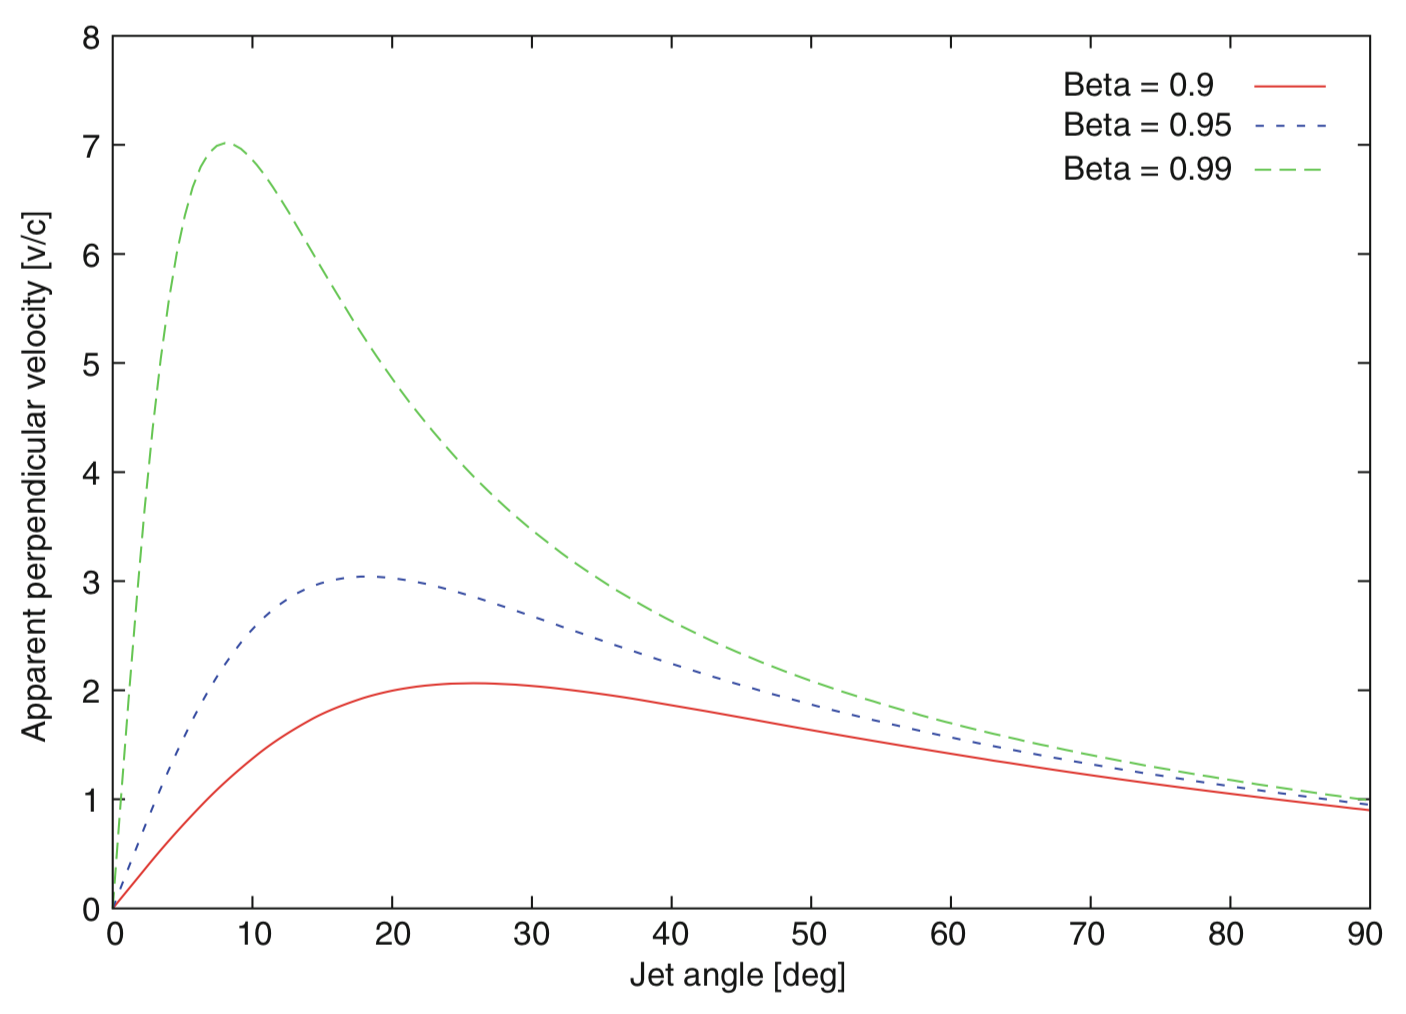
\includegraphics[width=12cm]{apparent_velocity.png}
\caption{The apparent jet velocity as a function of the angle to the line of sight for different jet velocities.
}\label{FIG:apparent_jet_velocity}
\end{center}
\end{figure}


The viewing angle at which a jet appears to have a maximal $v_\perp$ is found from $\dfrac{\dif v_\perp}{\dif \theta} = 0$ which gives $\cos \theta = \beta$.
\begin{equation}
v_{\perp, \rm max} = \gamma v ~.
\end{equation}



\cite{weekes2003very} The total energy ranges over three decades: from $5 \times 10^{51}$ to $3 \times 10^{54}$ erg. The time scale of the emission is very small so that the dimensions of the emitting regions must also be small, e.g. a $3$ ms flare indicates an emission region of $10^8$ cm. With such a high density, the photon-photon pair-production process would have such a large cross section that it would be impossible for the gamma rays to escape.

If there is beaming, then the total energy is considerably reduced, the absorption problem is reduced, and the ubiquitous bulk motion in a relativistic jet is invoked. Whereas the bulk Lorentz factor, $\Gamma$, in AGN had values of approximately $10$, to explain GRBs, $\Gamma$ must have values in excess of $100$. In this way the total energy emitted from the GRB can be reduced by a factor of $10^{2-3}$, i.e. to $10^{51}$ erg, comparable to that of a supernova explosion. GRBs must be much more frequent than was previously supposed. If the beam factor is $1/500$, then the real rate of GRBs may be $\approx 500/$day, instead of the observed $1/$day because the emission is only visible within the solid angle of $1/\Gamma$. However, the effect of collimation must also be taken into account.

The emission of the gamma radiation in GRBs is the result of a relativistic fireball. The shells of relativistic material are emitted into the interstellar medium in a succession of explosive events. As different shells interact, they produce shocks. The GRB is thought to be caused by these internal shocks. The afterglow is due to the external shock, the termination of the jet as it interacts with the surrounding interstellar medium. The source of the emission for both the prompt and delayed emission is the relativistic outflow in the jet and it occurs in regions that are optically thin so the gamma rays can escape. The observed x-ray, optical, and radio afterglow is synchrotron emission from the relativistic electrons.

\subsection{Photon arrival time from a moving source, Doppler shift, Lorentz invariance of power etc.}
\cite{2015PhR...561....1K} Consider \textcolor{blue}{a source moving with speed $v$, and corresponding Lorentz factor $\Gamma$, at an angle $\theta$ with respect to the line of sight to the observer located far away from the source}. \textcolor{red}{Two photons are emitted $\delta t^\prime$ apart in the source comoving frame}. In the lab frame (the frame in which the source is seen to move at speed $v$), the time interval of emitting these two photons is $\delta t = \Gamma \delta t^\prime$. The time difference for the arrival of these photons at the observer is given by (see Fig. \ref{FIG:photon-arrival})
\begin{align}
\nonumber \delta t_{\rm obs} &= \delta t +[d -v\cos \theta (\delta t)]/c -d/c \\
\nonumber &= \delta t (1 -v \cos \theta /c) \\
\nonumber &= \delta t^\prime \Gamma (1 -v \cos \theta /c) \\
&= \delta t^\prime \mathscr D^{-1} 
\label{observer-time}
\end{align}
where $d$ is the distance to the source,
\begin{equation}
\mathscr D = [\Gamma (1 -v \cos \theta /c)]^{-1}
\end{equation}
is the \textcolor{red}{Doppler factor}. For $\theta \ll 1$ and $\Gamma \gg 1$, the above expression for $\delta t_{\rm obs}$ can be approximated as
\begin{equation}
\delta t_{\rm obs} \approx \dfrac{\left[1 +(\theta \Gamma)^2\right]}{2\Gamma} \delta t^\prime = \dfrac{\left[1 +(\theta \Gamma)^2 \right]}{2 \Gamma^2} \delta t ~.
\end{equation}
The \textcolor{blue}{photon frequency in the observer frame, $\nu$}, can be expressed in terms of the \textcolor{blue}{comoving frame frequency $\nu^\prime$} using the standard Lorentz transformation of photon $4$-momentum in comoving frame - $\nu^\prime(1, \cos \theta^\prime, \sin \theta^\prime, 0)$ - to the lab frame 4-momentum $\nu(1, \cos \theta, \sin \theta, 0)$
\begin{align}
& \nu = \nu^\prime \Gamma (1 +v \cos \theta^\prime /c) \\
&\nu \cos \theta = \nu^\prime \Gamma (\cos \theta^\prime +v/c)
\end{align}
or
\begin{equation}
 \nu = \dfrac{ \nu^\prime}{\Gamma (1 -v \cos \theta /c)} \equiv  \nu^\prime \mathscr D ~,
\end{equation}
which is the standard \textcolor{red}{Doppler shift formula}.

\begin{figure}
\begin{center}
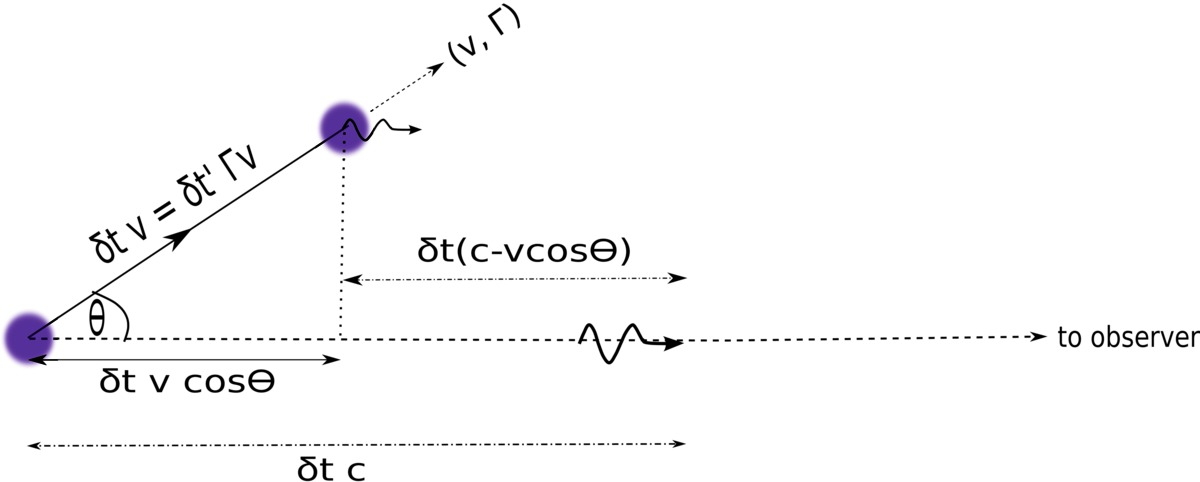
\includegraphics[width=12cm]{observed-pulse-duration.jpg}
\caption{The relation between pulse duration in source comoving frame, $\delta t'$, lab frame ($\delta t$), and the time interval for pulse received by a distant observer is shown in this figure. The source is moving with speed $v$ (Lorentz factor $\Gamma$), at an angle $\theta$ with respect to observer line of sight. One photon is emitted when the source was at the location at the left side of the figure. And a second photon is emitted $\delta t'$ later when the photon has already traveled a distance $c \delta t$ toward the observer, and the source is also a distance $v \cos\theta \delta t$ closer. The difference between these two distances is the time interval in the observer frame for the arrival of the two photons which is given by Eq. (\ref{observer-time}).
}
\label{FIG:photon-arrival}
\end{center}
\end{figure}


\subsubsection{Relativistic beaming of photons}
The transverse component of momentum does not change under Lorentz transformation, i.e. its comoving and lab frame values are the same
\begin{equation}
\nu \sin \theta = \nu^\prime \sin \theta^\prime ~\text{or}~ \sin \theta = \sin \theta^\prime /\mathscr D ~.
\end{equation}
For large $\Gamma$,  \textcolor{red}{$\theta \approx \theta^\prime /\Gamma$}, i.e. \textcolor{red}{photons are focused in the forward direction such that the angular size of the photon beam in the lab frame is smaller than it is in the comoving frame by a factor $\sim \Gamma$}. The  \textcolor{red}{solid angle for a conical beam of photons in lab frame is smaller than in the comoving frame by a factor $\sim \Gamma^2$}. The \textcolor{red}{Lorentz transformation of solid angle} is:
\begin{equation}
\dif \Omega = \sin \theta \dif \theta \dif \phi = \sin \theta^\prime \dif \theta^\prime \dif \phi^\prime /\mathscr D^2 = \dif \Omega^\prime /\mathscr D^2
\label{equ:solid_ang}
\end{equation}
The  \textcolor{red}{power (Power is defined as the frequency integrated total energy radiated per unit time over $4\pi$ steradians.) radiated by a particle is Lorentz invariant when the radiation beam is symmetric under parity transformation in particle rest-frame}, i.e. the energy radiated per unit solid angle in directions $(\theta, \phi) \& (\pi -\theta, \pi+\phi)$ are equal. Consider the $4$-momentum carried away by photons emitted in time interval $\delta t^\prime$ in the source frame, which is: $P^\prime \delta t^\prime(1,0,0,0)$; where  \textcolor{blue}{$P^\prime$ is the power in source comoving frame}, and the space components are zero because of parity symmetry. The $4$-momentum and the elapsed time in the lab frame are: $\Gamma P^\prime \delta t^\prime(1, v, 0, 0), \Gamma \delta t^\prime$. Hence the power in the lab frame is $P = P^\prime \Gamma  \delta t^\prime/(\Gamma  \delta t^\prime) = P^\prime$.

\subsubsection{Transformation of specific luminosity and specific intensity}
The Lorentz transformation of luminosity. Consider a source that is spherically symmetric and is expanding with Lorentz factor (LF) $\Gamma$. The observed specific luminosity, $L_\nu$, is the total energy that flows through a surface enclosing the source per unit time and frequency. Thus, it follows that
\begin{equation}
L_\nu = \dfrac{\dif E}{\dif \nu \dif t_{\rm obs}} = \Gamma \dfrac{\dif E^\prime}{\dif \nu^\prime \dif t^\prime} = \Gamma  L^\prime_{\nu^\prime} ~,
\end{equation}
where we made use of $\dif \nu \dif t_{\rm obs} = \dif \nu^\prime \dif t^\prime$, and $E = \Gamma E^\prime$ when the $3$-momentum vector is zero as it must for a spherically symmetric radiation source.

The \textcolor{red}{specific intensity} is defined as \textcolor{blue}{flux per unit frequency and per unit solid angle carried by photons traveling within a narrow conical beam with its axis perpendicular to surface $\dif A$}, i.e.
\begin{equation}
I_\nu \equiv \dfrac{\dif E}{\dif \nu \dif t_{\rm obs} \dif A \dif \Omega} ~. 
\end{equation}
Considering that $E$ transforms as $\nu$, $\dif \Omega$ transformation is given by Eq. (\ref{equ:solid_ang}), and \textcolor{red}{$\dif \nu \dif t_{\rm obs} \dif A$ is Lorentz invariant}, 
\begin{equation}
I_\nu = \mathscr D^3 I^\prime_{\nu^\prime} ~.
\end{equation}

\subsubsection{Observed lightcurve from a source that is suddenly turned off}
Transient sources such as GRBs can turn off rapidly on a time scale of a second or less. Consider a relativistic, conical, optically thin source moving with LF $\Gamma$ turns off abruptly, and calculate how the flux declines with time as seen by a far away observer in a fixed frequency band.

Consider the source to be a thin shell, and points in the source are specified by $(r, \theta, \phi)$ where angle $\theta$ is measured with respect to the line of sight to the observer. The source turns off suddenly when it is at radius $r = R_0$. Photons released at $(r = vt, \theta, \phi)$ arrive at the observer with a time delay with respect to a photon emitted at $r = 0$ of
\begin{equation}
t_{\rm obs} = t - r \cos \theta/c =t(1- v\cos \theta/c) = t/(\Gamma \mathscr D) ~.
\label{t_obs}
\end{equation}
Calculate the lightcurve at frequency $\nu$ from the source after time $t_{0, \rm obs} \approx R_0/(2c\Gamma^2)$ which corresponds to the arrival of photons from $(R_0, 0, 0)$ at the observer. At $t_{\rm obs} > t_{0, \rm obs}$ the observer sees photons which left the source when $r < R_0$ as determined by Eq. (\ref{t_obs}). The time dependence of the observed flux, when the intrinsic spectrum is $I^\prime_{\nu^\prime} = I^\prime \nu^{\prime, -\beta}$, follows from the Lorentz transformation of specific intensity. At any given observer time $t_{\rm obs} > t_{0, \rm obs}$ we receive radiation from $\theta > \theta_t$; where $\theta_t$ is the angle corresponding to time $t_{\rm obs}$ such that $t_{\rm obs} = R_0 (1/v -\cos \theta_t /c)$. Considering that the observed flux is proportional to the integral of $I_\nu$ over the solid angle of the source, $f_\nu \propto \int_{\theta_t} \dif \theta \sin \theta \mathscr D^{-(3+\beta)}$. Or $f_\nu \propto (1 - v \cos \theta_t /c)^{-(2+\beta)} \propto t^{-(2+\beta)}_{\rm obs}$. 

The specific flux in observer frame from a relativistic source of comoving specific intensity $I^\prime_{\nu^\prime}$ and spectrum $\propto \nu^{\prime -\beta}$ is given by
\begin{equation}
f_\nu(t_{\rm obs}) = \int \dif \Omega_{\rm obs} I_\nu \cos \theta_{\rm obs} = 2\pi \int \dif \theta_{\rm obs} \dfrac{I^\prime_{\nu^\prime_0} \nu^{\prime \beta}_0 \sin 2\theta_{\rm obs} [(1+z) \Gamma]^{-(3+\beta)} }{2\nu^\beta [1-v \cos(\theta +\theta_{\rm obs})/c]^{3+\beta} }~,
\end{equation}
where $\nu^\prime_0$ is a frequency that lies on the power law segment of the spectrum for $I^\prime_{\nu^\prime}$, and we made use of the Lorentz transformation of specific intensity to obtain the last part of the above equation. The factor $(1 + z )^{3+\beta}$ in the above equation takes into account redshift of frequency for a source at $z$.

Using the law of sine for a triangle, $\sin \theta/d_A = \sin \theta_{\rm obs}/r$, the above integral is transformed to 
\begin{equation}
f_\nu \approx \dfrac{2\pi I^\prime \nu^\prime_0 \nu^{\prime \beta}_0 \nu^{-\beta} }{[(1+z) \Gamma]^{3+\beta} } \left(\dfrac{R_0}{d_A} \right)^2 \int_{\theta_t}^{\pi/2} \dif \theta \dfrac{\sin \theta \cos \theta}{(1-v\cos \theta/c)^{3+\beta} } ~.
\end{equation}
We replaced $\theta + \theta_{\rm obs}$ in the denominator with $\theta$ since $\theta_{\rm obs} \ll \theta$. The above integral is straightforward to carry out and yields
\begin{equation}
f_\nu(t_{\rm obs}) \propto (1-v\cos \theta_t/c)^{-(2+\beta)} \nu^{-\beta} \propto t_{\rm obs}^{-(2+\beta)} \nu^{-\beta} ~.
\end{equation}
Thus, the observed radiation does not drop to zero as soon as the source is turned off, but the flux declines rapidly with time and eventually vanishes when $\theta_t$ exceeds the angular size of the source ($\theta_j$).

\subsection{Synchrotron radiation}
Consider an electron of Lorentz factor $\gamma_e$, and speed $v_e$, moving perpendicular to the magnetic field of strength $B$. 
The electric field in the electron rest frame is $E = \gamma_e v_e B/c$, and hence according to the Larmor's formula the power 
radiated due to electron acceleration in this electric field is 
\begin{equation}
    P_{syn} = {2 q^4 E^2 \over 3 c^3 m_e^2} = {2 q^4 B^2 \gamma_e^2
  v_e^2\over 3 c^5 m_e^2} = \sigma_T B^2 \gamma_e^2 v_e^2/(4\pi c),
  \label{P_syn}
\end{equation}
where $\sigma_T = 8\pi q^4/(3 m_e^2 c^4)$ is the Thomson cross section. Since electric dipole radiation has parity symmetry, $P_{syn}$ is a Lorentz invariant quantity, and hence the above equation gives the correct synchrotron power from an electron as viewed in the lab frame. The average power per electron, for isotropic pitch angle distribution, is smaller than the above expression by a factor $3/2$.

\begin{figure}
\begin{center}
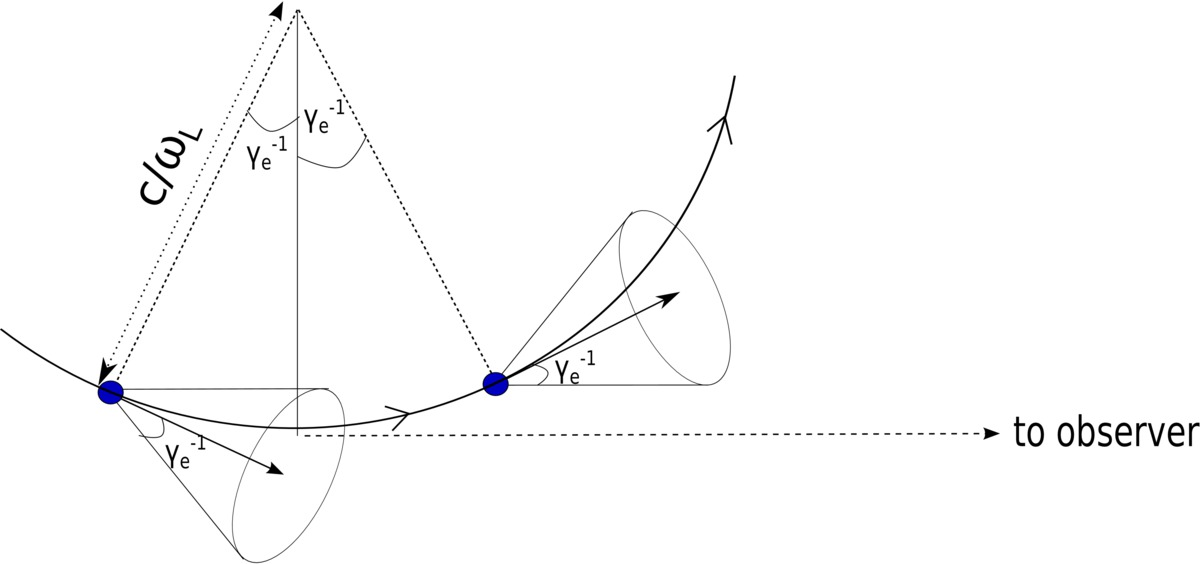
\includegraphics[width=12cm]{synchrotron-radiation.jpg}
\caption{The figure shows a segment of electron orbit that is moving in magnetic field with LF $\gamma_e$. Radiation from the electron is received by a distant observer only for a small segment of the orbit when the electron's velocity vector lies within $\gamma_e^{-1}$ of the observer line of sight as a result of the beaming of photons in the forward direction in the lab frame (radiation in electron comoving frame is dipolar which covers almost $4\pi$ steradians). The observed synchrotron peak frequency for emission from this electron follows from this simple property (eq. \ref{syn_omega}).
}\label{FIG:relativistic_beaming}
\end{center}
\end{figure}

The Larmor frequency of the electron (or its angular speed) is
\begin{equation}
   \omega_L = {q B \over \gamma_e m_e c}.
\end{equation}
Due to relativistic beaming of photons, radiation from the electron that a distant observer receives is confined to the duration when the electron velocity vector lies within an angle $\gamma_e^{-1}$ of the observer line of sight (fig. \ref{FIG:relativistic_beaming}).
The fraction of orbital time when this condition is satisfied is
$\sim 1/\pi\gamma_e$, and therefore the duration of the radiation
pulse received by the observer in each orbit is:
\begin{equation}
   \delta t_{obs} \sim {2\over \gamma_e\omega_L} {1\over 2\gamma_e^2}
        \sim {m_e c \over q B \gamma_e^2},
\end{equation}
where we used equation (\ref{observer-time}) that relates the
comoving time, $\delta t' = \delta t/\gamma_e$, to the observer
frame time duration for photon pulse arrival. The inverse of this
time is the characteristic frequency for synchrotron radiation 
which is given by
\begin{equation}
    \omega_{syn} \sim {q B \gamma_e^2\over m_e c} \quad{\rm and}\quad
     \nu_{syn} = {\omega_{syn} \over 2\pi} \sim {q B \gamma_e^2\over 2\pi 
   m_e c}, 
  \label{syn_omega}
\end{equation}
where $\nu_{syn}$ is the cyclic frequency. A more precise treatment
has an additional factor $(3/2)\sin \alpha$; $\alpha$ is the pitch angle 
between the electron's velocity and the magnetic field.
The synchrotron spectrum peaks at $\sim\nu_{syn}$. The spectrum 
below the peak scales as $P_{syn}(\nu) \propto \nu^{1/3}$ (this behavior is 
determined by the Fourier transform of the synchrotron pulse profile),
and it declines exponentially for $\nu>\nu_{syn}$ (see Fig. 
\ref{FIG:syn_spec}); we
refer to \cite{rybicki79} for the calculation of synchrotron
spectrum. The power per unit frequency $P_{syn}(\nu)$ 
at the peak of the spectrum is
\begin{equation}
   P_{syn}(\nu_{syn}) \sim P_{syn}/\nu_{syn} \sim {\sigma_T B m_e c^2
     \over 2 q}.
    \label{p_syn_peak}
\end{equation}

\begin{figure}
\begin{center}
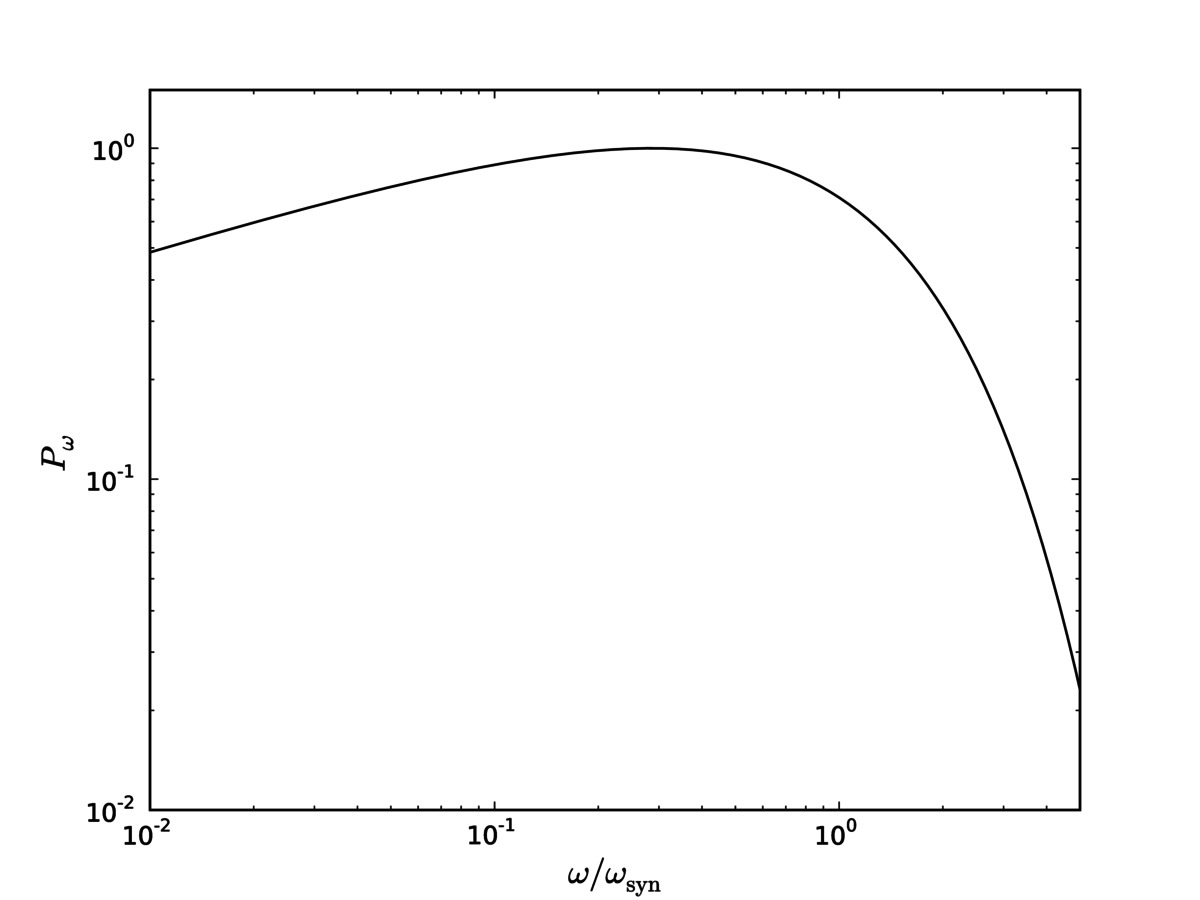
\includegraphics[width=11cm]{synchro_spec1.jpg}
\caption{This figure shows the synchrotron spectrum for a single
electron; the x-axis is frequency in units of $\omega_{syn}$ (see
eq. \ref{syn_omega}), and the flux is normalized to unity at the peak.
}\label{FIG:syn_spec}
\end{center}
\end{figure}

The synchrotron spectrum for a power-law distribution of electrons, 
$d n_e/d\gamma_e \propto \gamma_e^{-p}$, is $f_\nu\propto\nu^{-(p-1)/2}$.
This follows from adding up contributions to the specific flux at $\nu$
from those electrons with LF larger than
\begin{equation}
   \gamma_\nu \sim \left( {2\pi\nu m_e c \over q B}\right)^{1/2},
  \label{gamma_nu}
\end{equation}
and that leads to
\begin{equation}
   f_\nu = \int_{\gamma_\nu}^\infty d\gamma_e {d n_e\over d\gamma_e}
        P_{syn}(\nu) \propto \nu^{-(p-1)/2},
\end{equation}
where we made use of $P_{syn}(\nu) \propto (\nu/\nu_{syn})^{1/3}$ for
$\nu < \nu_{syn}$, and equation (\ref{syn_omega}) for $\nu_{syn}$.

\subsubsection{Effect of synchrotron cooling on electron distribution}

Another characteristic synchrotron frequency is associated with the
cooling of electrons ($\nu_c$). Let us consider that electrons are
accelerated at some time, and then cool via synchrotron radiation
for time duration $t_0$. Electrons with LF $\leqslant \gamma_c$ 
(defined below) lose a significant fraction of their energy 
during this time and their LF drops below $\gamma_c$
\begin{equation}
   {d m_e c^2 \gamma_e \over dt} = - {\sigma_T\over 6\pi} B^2 
    \gamma_e^2 c \quad\quad {\rm or} \quad \quad \gamma_c \sim 
    {6\pi m_e c\over \sigma_T B^2 t_0}.
  \label{gam_c}
\end{equation}
The synchrotron frequency corresponding to this LF is defined as
the synchrotron cooling frequency:
\begin{equation}
   \nu_c \equiv {3 q B \gamma_c^2\over 4\pi m_e c} \sim 
       {27 \pi q m_e c\over \sigma_T^2 B^3 t_0^2}.
  \label{nu_c}
\end{equation}
The power-law index of the synchrotron spectrum changes at $\nu_c$ due to the fact that electron distribution function for $\gamma_e >\gamma_c$ is modified as a result of loss of energy. This can be seen from the continuity equation for electrons in the energy space:
\begin{equation}
    {\partial \over \partial t}{d n_e\over d\gamma_e} + {\partial 
    \over \partial \gamma_e} \left[ \dot{\gamma_e} {d n_e\over 
   d\gamma_e}\right] = S(\gamma_e),
\end{equation}
where $\dot{\gamma_e} = - \sigma_T B^2 \gamma_e^2/(6\pi m_e c)$ is the rate of change of $\gamma_e$ due to synchrotron loss, and $S(\gamma_e)$ is the rate at which electrons with LF $\gamma_e$ are injected into the system. The continuity equation has a steady state solution ($\partial/\partial t = 0$) for time independent magnetic field which is: $d n_e/d\gamma_e\propto \dot{\gamma_e}^{-1} \propto \gamma_e^{-2}$ for $\gamma_c < \gamma_e < \gamma_m$; where $\gamma_m$ is the minimum LF of injected electrons i.e. $S(\gamma_e) = 0$ for $\gamma_e < \gamma_m$. The synchrotron spectrum corresponding to this segment of electron distribution function is $f_\nu \propto \nu^{-1/2}$. For a time dependent magnetic field the distribution function is not a power law function of $\gamma_e$ with index $2$, and in general its shape evolves with time.

For $\gamma_e > \gamma_c > \gamma_m$, the solution of the continuity equation is $d n_e/d\gamma_e \propto \gamma_e^{-p-1}$ in the steady state (for constant $B$). And the corresponding synchrotron spectrum is $f_\nu \propto \nu^{-p/2}$.

\subsubsection{Synchrotron self-absorption frequency}
Yet another characteristic frequency, $\nu_a$, corresponds to the case where absorption of photons by the inverse-synchrotron process becomes important. The easiest way to determine $\nu_a$ is by the application of Kirchhoff's law -- the emergent specific flux cannot 
exceed the black-body flux corresponding to the appropriate electron temperature which is
\begin{equation}
 k_B T \approx {\rm max} (\gamma_a, {\rm min}[\gamma_m,\gamma_c]) m_e c^2/2.7
\end{equation}
where $\gamma_m$, $\gamma_c$ and $\gamma_a$ are electron Lorentz factors
corresponding to synchrotron frequencies $\nu_m$, $\nu_c$ and $\nu_a$,
respectively, and $k_B$ is Boltzmann constant. The synchrotron self-absorption 
frequency ($\nu_a$) is the frequency where the emergent synchrotron flux 
is equal to the black-body flux:
\begin{equation}
   {2 m_e c^2 {\rm max}(\gamma_a,{\rm min}[\gamma_m,\gamma_c]) 
\nu_a^2 \over 2.7 c^2} \approx
         {\sigma_T B m_e c^2 N_>\over 4\pi q}
\label{nu_a}
\end{equation}
where the left side of this equation is the Planck function in the Rayleigh-Jeans limit, and $N_>$ is the column density of electrons with LF larger than ${\rm max}(\gamma_a,{\rm min} [\gamma_m,\gamma_c])$.

The emergent synchrotron spectrum for a distribution of electrons depends on the ordering of these characteristic frequencies. Spectra for two particular orderings are shown in fig. \ref{FIG:synchro_spectrum2}.

\begin{figure}
\begin{center}
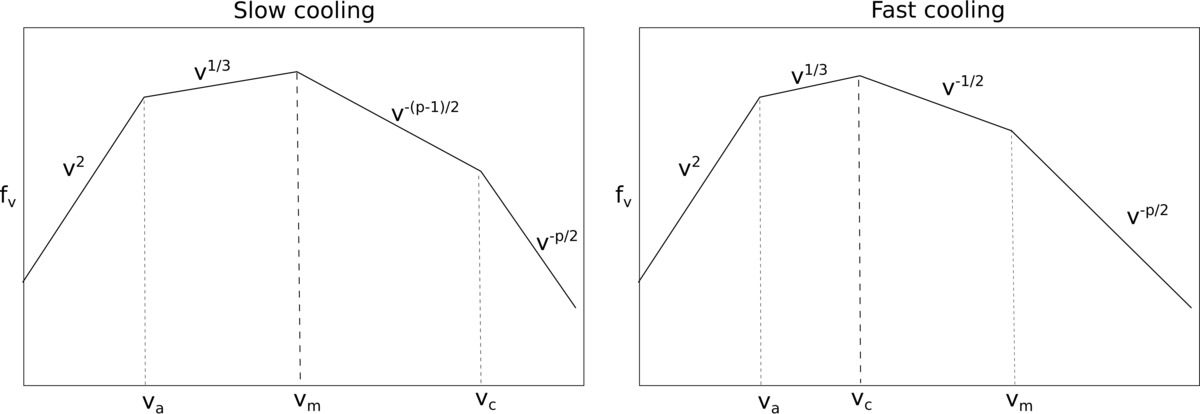
\includegraphics[width=16cm]{synchro_spec2.jpg}
\caption{Synchrotron spectrum for the case where $\nu_a<\nu_m<\nu_c$ is shown in the left panel, and for the case $\nu_a<\nu_c<\nu_m$ in the right panel.
}
\label{FIG:synchro_spectrum2}
\end{center}
\end{figure}

\subsubsection{Maximum energy of synchrotron photons}
\label{synch_rad_max}

Charged articles are accelerated as they travel back and forth across a shock front via the first order Fermi process. They gain energy by a factor $\sim 2$ each time they are scattered from one side to the other of a relativistic shock front. The maximum synchrotron frequency for an electron in this case turns out to be about $50 \Gamma$ MeV, and for a proton it is a factor $m_p/m_e$ larger; $\Gamma$ is the Lorentz factor of shocked plasma with respect to the observer, and $m_p$ is proton mass.

The minimum time required for acceleration of a charged particle of mass $m$ while crossing a shock front is of the order of the Larmor time $t'_L = m c\gamma/(qB')$; where $\gamma$ is LF of the particle in the shock comoving frame, and prime ($'$) refers to quantity measured in the rest frame of the shocked fluid. The particle should not lose more than half its energy to synchrotron radiation in time $t'_L$, otherwise it will never get accelerated to LF $\gamma$. This implies that $4 q^4 B'^2\gamma^2 t'_L/(9 m^2 c^3) < m c^2 \gamma/2$ or $ qB'\gamma^2/(2\pi m c) < 9mc^3/(16\pi q^2)$. The left side of the last inequality is the synchrotron frequency for the particle, and the right side depends on the particle's mass. So we find that the maximum synchrotron photon energy for an electron (proton) is $\sim$50 MeV (100 GeV) in shocked fluid comoving frame under the optimistic Bohm diffusion limit.

It is possible to violate this limit, by a factor of a few at least, when the magnetic field is highly inhomogeneous down stream of the shock front; synchrotron photons produced when a particle is passing through a region of much higher-than-average magnetic field can have energy larger than the limit described above.

\subsection{Inverse-Compton radiation}

When a photon of frequency $\nu$ is scattered by an electron of larger 
energy, the photon gains energy in this process on the average.  
If the electron Lorentz factor is $\gamma_e$, and $h \nu \gamma_e \ll
m_e c^2$, then the average frequency of scattered photon is 
$\nu_s\sim \nu\gamma_e^2$. This is easy to see by viewing the process
from the rest frame of the electron where the angle-averaged 
frequency of the incident photon is $\nu'\sim \nu\gamma_e$ 
(see eq. \ref{doppler} for relativistic Doppler shift). For
$h\nu'\ll m_e c^2$ the scattering is elastic -- the electron
recoil can be neglected -- so that the scattered photon has frequency
$\nu'$ (in electron rest frame) and its angular probability 
distribution is a dipole function.  Transforming the frequency 
of the scattered photon back to the original frame introduces another 
Lorentz boost and that results in $\nu_s \sim \nu\gamma_e^2$.

Consider next an electron moving through a radiation field
where the energy density in photons is $u_\gamma$. The power in 
IC-scattered photons, $P_{\rm ic}$, follows from the energy boost 
by a factor $\gamma_e^2$ for each photon (independent of 
photon energy for the case where $h\nu\gamma_e \ll m_e c^2$
that we are considering here):
\begin{equation}
   P_{\rm ic} \sim \sigma_T \int d\nu {u_\nu c\over h\nu} h\nu\gamma_e^2
     \sim \sigma_T u_\gamma \gamma_e^2 c,
  \label{P_ic1}
\end{equation}
where $u_\nu d\nu$ is energy density in photons of frequency between $\nu$ and $\nu+\dif \nu$; $\int d\nu \, u_\nu = u_\gamma$.
We see from equations (\ref{P_syn}) and (\ref{P_ic1}) that the ratio of synchrotron and IC powers is $u_B/u_\gamma$; where $u_B = B^2/8\pi$ is the energy density in magnetic field.

A particularly important case of IC radiation is when seed photons
are produced by the synchrotron process, i.e. electrons that produce
seed photons also IC scatter them to typically much larger energies. 
This process --- called synchrotron-self-Compton or SSC --- could be 
important for GRBs and other relativistic sources. 
The relative importance of synchrotron and IC processes for extracting
energy from a population of energetic electrons is specified by the 
Compton Y parameter. Energy density in photons for the synchrotron process is:
\begin{equation}
   u_\gamma = \int dr \int d\gamma_e\, {P_{syn}\over c} {d n_e\over 
     d\gamma_e} = {\sigma_T (\delta R) B^2 \over 6\pi} 
     \int d\gamma_e\, \gamma_e^2
      {d n_e\over d\gamma_e} = {\sigma_T (\delta R) n_e B^2 \over 6\pi} 
      \langle \gamma_e^2 \rangle,
\end{equation}
where $\delta R$ is the radial width of the source, and 
\begin{equation}
   \langle \gamma_e^2 \rangle \equiv {1\over n_e} \int d\gamma_e\, 
   \gamma_e^2 {d n_e\over d\gamma_e}.
\end{equation}
Making use of the expression for $u_\gamma$ for synchrotron radiation
we find the Compton-Y parameter to be
\begin{equation}
    Y \sim P_{ic}/P_{syn} \sim \tau_e \langle \gamma_e^2\rangle, 
   \quad\quad{\rm where} \quad\quad
          \tau_e = \sigma_T (\delta R) n_e
  \label{Y-expression1}
\end{equation}
is the optical depth of the source to Thomson scattering. 

\subsubsection{IC spectrum}
The spectrum of IC radiation is obtained by convolving electron distribution with the seed photon spectrum 
\begin{equation}
f_{\rm ic} (\nu_{\rm ic}) \approx \dfrac{3 \sigma_T(\delta R)}{4} \int \dif \nu \dfrac{\nu_{\rm ic}}{\nu^2} f_{\rm syn}(\nu) \int \dfrac{\gamma_{\rm e}}{\gamma_{\rm e}^2} \dfrac{\dif n_{\rm e}}{\dif \gamma_{\rm e}} F\left(\dfrac{\nu_{\rm ic}}{4 \gamma_{\rm e}^2 \nu} \right) ~,
\end{equation}
where
\begin{equation}
F(x) \approx \dfrac{2}{3} (1-x) ~, ~~ x \equiv \dfrac{\nu_{\rm ic}}{4 \gamma_{\rm e}^2 \nu} ~.
\end{equation}
It follows from these equations that the IC spectrum, $f_{\rm ic} (\nu_{\rm ic})$, for a $\delta$-function seed photon spectrum (where photons have frequency $\nu_0$), and a power-law distribution of electrons with index $p$ which is cutoff at the low energy end at $\gamma_m$, is proportional to $\nu_{\rm ic}$ for $\nu_{\rm ic} < 4 \gamma_{\rm m}^2 \nu_0$. Therefore, the low energy part of IC spectrum can be significantly harder than the hardest possible synchrotron spectrum ($\nu^{1/3}$) when synchrotron-self-absorption is negligible. At higher photon energies, $\nu_{\rm ic} > 4 \gamma_{\rm m}^2 \nu_0$, the IC spectrum has an asymptotic power-law index $\nu^{-(p-1)/2}_{\rm ic}$, same as the spectrum for the synchrotron process.

\subsubsection{IC in Klein-Nishina regime}
When photon energy in electron comoving frame approaches (or exceeds) $m_{\rm e}c^2$ two effects become important. One of which is that the electron recoil in the scattering can no longer be ignored. The other effect is that the cross-section is smaller than $\sigma_T$ and it decreases with increasing photon energy as $\sim \nu^{-1}$. One simple consequence of the recoil effect is that the energy of the scattered photon is limited to $\sim m_{\rm e} c^2 \gamma_{\rm e}/2$ (and is no longer $\sim \nu_0 \gamma_{\rm e}^2$) which is obvious from energy conservation.

Photo-pion process refers to the production of pions ($\pi^0, \pi^+$ and $\pi^-$) in collisions of photons with protons; charge conservation requires that $\pi^-$ is produced with at least one $\pi^+$. The decay of $\pi^+$ produces positrons of very high LF which can then produce high energy photons via the synchrotron process. A neutral pion $\pi^0$ can directly decay into two photons. The photo-pion process is likely to be important in those situations where electrons are unable to be accelerated efficiently to very high LFs whereas protons are. It also offers a way to beat the well known limit on the maximum synchrotron photon energy of about $50 \Gamma$ MeV for shock accelerated electrons.

The delta resonance for photon-proton interaction, $p + \gamma \rightarrow \Delta^+$, has the largest cross section, $\sigma_{\gamma p} = 5\times 10^{-28}$ cm$^2$, and the lowest energy threshold - $\sim 200$ MeV for photon in proton rest frame - of the photo-proton resonances, and is therefore the most important photo-pion interaction to consider for many astrophysical systems. The delta resonance has two main decay channels: $\Delta^+ \rightarrow \pi^+ + n$ and $\Delta^+ \rightarrow \pi^0 + p$. The neutral pions quickly decay in $8.4 \times 10^{-17}$ s (in their rest frame) to two photons, and the outgoing $\gamma$-ray energy is at least $67$ MeV (in pion rest frame).

The $\Delta^+$ decays in $2.6 \times 10^{-8}$ s to $\mu^+ \& \nu_{\mu}$, and the anti-muon subsequently decays as $\mu^+ \rightarrow e^+ + \bar{\nu}_\mu + \mu_{\rm e}$. The isospin conservation gives a branching ratio for $\pi^+ : \pi^0$ decay channels of $\Delta^+$ to be $1 : 2$. However, when contributions from all the possible resonances as well as the direct pion production are included the ratio of charged pions to neutral pions is actually closer to $2 : 1$. 

Another relevant process is the Bethe-Heitler pair production process $p + \gamma \rightarrow p + e^+ + e^-$.
































\section{Afterglow theory}

\cite{courvoisier2012high} The \textcolor{blue}{optical afterglows} give measurements of the redshifts of the GRBs, and allow us to get very precise positions from which is possible to find the environment of the bursts. It is found that they occur in galaxies, and are associated in particular with star formation regions.

In a few cases a supernova has been associated with the burst position and epoch. This association is based on the coincidence between a GRB and the detection of a supernova that seems to have exploded at the same epoch and in the same location of the sky. In some cases the optical spectrum of the burst afterglow emission has also been found to be similar to that of some categories of supernovae. These observations suggest that at least some GRBs are associated with core collapse supernovae. Only long GRBs have so far been associated one way or another with supernovae. However, such an association has to date not been possible for short GRBs. One may therefore conjecture that \textcolor{red}{long GRBs are associated with core collapse events}, and that \textcolor{red}{short GRBs are associated with the merger of two neutron stars}. 

Not all GRBs have optical afterglow emission. Burst for which optical emission has been looked for but not observed are referred to as ``dark". This may be due to the fact that the progenitor resides in a gas and dust rich medium that is optically thick to optical radiation, and only transparent in the hard X-rays. At the other extreme, some GRBs are very bright, having reached optical magnitudes accessible with the naked eye.

The observation of the light curve of the afterglows offers the interesting possibility of measuring the opening angle of the jet that underlies the GRB. The behaviour of the gamma factor in the jet as a function of time can be estimated assuming an adiabatic expansion. It is found that $\gamma \propto t^{-3/8}$. Relativistic aberration confines the angle in which the radiation from an accelerated charge is observable to a cone of opening angle $1/\gamma$. Assuming a spherical relativistically moving photosphere, only a fraction $1/\gamma^2$ of the sphere surface emits radiation observable by a distant observer. Thus as time proceeds and $\gamma$ decreases, a larger and larger fraction of the photosphere contributes to the observed flux. This increasing surface is proportional to $1/\gamma^2 \propto t^{3/4}$. At some time the whole jet is encompassed by the visibility cone. This happens for an observer on the axis of the jet when the jet opening angle $\theta_c \simeq 1/\gamma$. For subsequent times, the area from which the flux reaches the observer does no longer increase. The slope of the light curve will, therefore, steepen by $-3/4$. The behaviour of the light curve will then reflect the emissivity of the whole jet rather than that of the jet fraction which increasingly contributes to the observed flux. A direct exploitation of this fact is made difficult by the complex behaviour of the intrinsic emission of the GRB afterglow. 

\cite{weekes2003very} The GRB sources appear to be in star-forming regions, not far from the center of the galaxy; the galaxies are blue and not very bright. The x-ray afterglow is observed to decay with time, $t$, as $F_x \propto t^{-(1-1.5)}$. The spectrum is softer than that in the prompt emission. Only in half the cases where a definite x-ray afterglow was measured is there detectable optical emission. This is always faint ($\approx 20 m_v$) and decays rapidly ($F_0 \propto t^{-(0.8-2.2)}$). The absence of optical emission is clearly significant and several theories have been advanced to explain these `dark' GRBs. The radio afterglows are particularly interesting because the rapid variability (scintillation on passing through the interstellar medium) is observed initially and this sets a limit to the maximum angular size of the afterglow region. Typically, the scintillation ceases about a month after the burst. For the sources with measured $z$, it is then possible to deduce the linear dimension of the source and, knowing the time since the GRB occurred, the velocity of the expanding fireball. It is these data that are used to calculate the total energy associated with each GRB where beaming is assumed














































%%%%%%%%%%%%%%%%%%%%%%%%%%%%%%%%%%%%%%%%%%%%%%%%%%%%%%%%%%%%%%%%%%%%%%
\bibliographystyle{unsrt_update}
\bibliography{ref}
%%%%%%%%%%%%%%%%%%%%%%%%%%%%%%%%%%%%%%%%%%%%%%%%%%%%%%%%%%%%%%%%%%%%%%


\end{document}